\clearpage
\section{Введение}

Ежегодно растет количество публикаций, посвященных глубокому обучению (рис.
\ref{fig:publications}). Росту популярности способствует постоянный рост
вычислительных возможностей, доступных исследователям. Об увеличивающемся
потенциале компьютерных технологий говорит Раджа Кодури (англ. 
\textit{Raja Koduri}), старший вице-президент и главный архитектор компании
Intel, в своем докладе на конференции HPC DevCon 2019
\footnote{Запись доклада доступна по адресу https://www.youtube.com/watch?v=-kWiRrf2o6Q}.
В то же время, по его словам, выполнение закона Мура\footnote{Закон Мура -- 
эмпирическое наблюдение, сделанное сооснователем Intel Гордоном Муром, согласно
которому количество компонентов на интегральной схеме удваивается каждые 18
месяцев.} во многом обеспечивается за счет развития специализированных
ускорителей: GPU, FPGA, DSP, VPU, TPU и т.д. Такой <<зоопарк>> аппаратных
средств требует особых инструментов разработки. Это послужило толчком к появлению
таких технологий, как CUDA и OpenCL.
\begin{figure}[h]
\centering
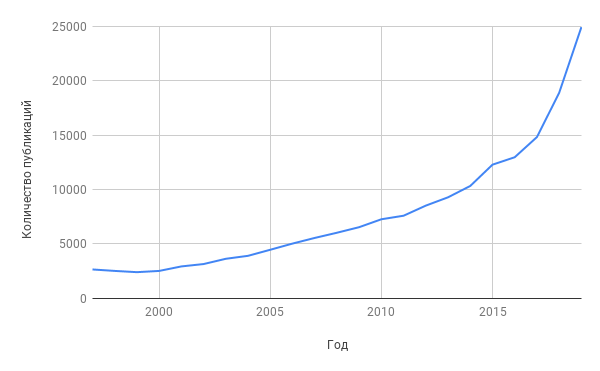
\includegraphics[width=0.8\textwidth]{publications_chart}
\caption{Динамика популярности поисковых запросов. Источник: sciencedirect.com}
\label{fig:publications}
\end{figure}
\begin{figure}[h]
\centering
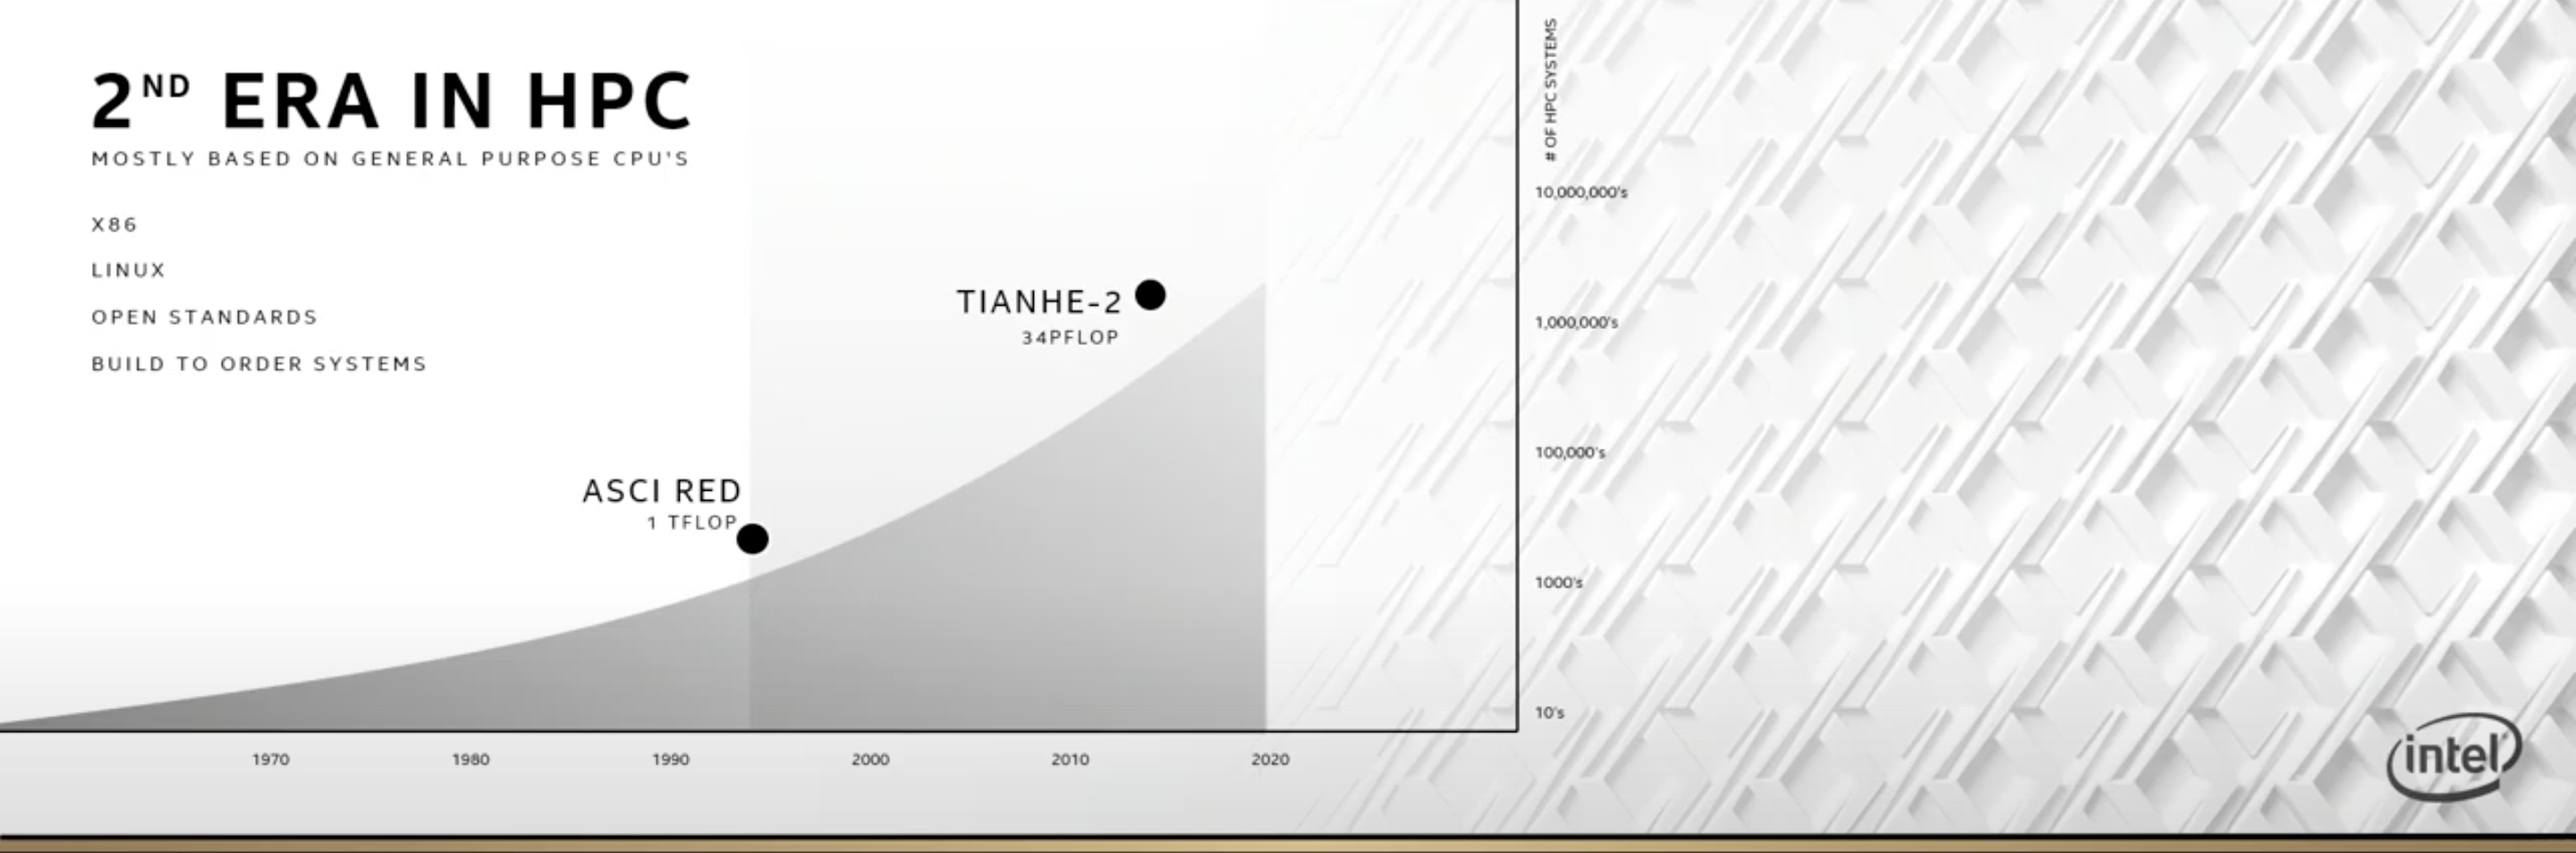
\includegraphics[width=\textwidth]{supercomputer_perf}
\caption{Рост вычислительной мощности суперкомпьютеров. Источник: Intel}
\label{fig:publications}
\end{figure}

Являясь инструментом решения многих прикладных задач, нейронные сети привлекают
не только исследователей, но также бизнес и просто энтузиастов. Чтобы сделать
глубокое обучение более доступным, были разработаны так называемые фреймворки
глубокого обучения -- программные средства, предоставляющие абстракцию над
аппаратным обеспечением. График \ref{fig:search_queries} показывает популярность
различных поисковых запросов. Из него можно видеть, что в то время, как интерес
к технологиям программирования ускорителей падает, растет популярность
фреймворков.
\begin{figure}[h]
\centering
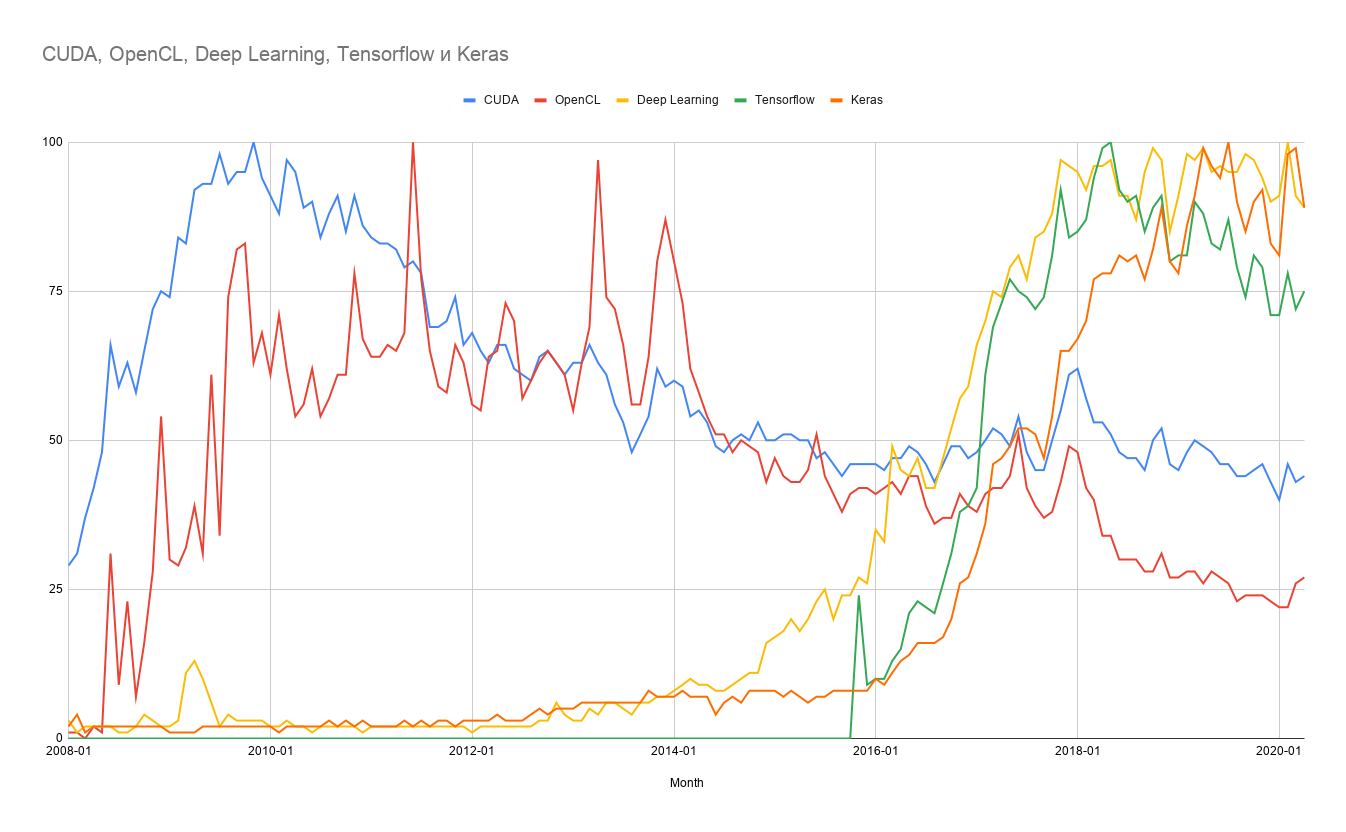
\includegraphics[width=\textwidth]{search_queries}
\caption{Динамика популярности поисковых запросов}
\label{fig:search_queries}
\end{figure}

В то же время, распространенной практикой становится применение компиляторных
технологий в машинном обучении. Это вызвано постоянно растущим количеством
различных ускорителей и аппаратных платформ. Примером таких продуктов могут быть
Glow от Facebook, MLIR и XLA от Google, PlaidML и nGraph от Intel.

Изложенные выше факты говорят об актуальности настоящей работы.

Целью данной работы является исследование применения технологий разработки и
построения компиляторов в задачах машинного обучения.

Исходя из цели работы, поставлены и решены следующие задачи:
\begin{enumerate}
\item Исследование архитектурных особенностей и возможностей современных
      фреймворков для задач искуственного интеллекта;
\item Изучение основных принципов построения современных компиляторов;
\item Разработка компилятора графа вычислений, как базоваого элемента для
      построения фреймворков искусственного интеллекта.
\end{enumerate}

В работе использовались научные труды отечественных и зарубежных специалистов.

Создание компилятора позволит обеспечить вычислительную поддержку математического
аппарата, используемого при построении нейронных сетей, а так же продемонстрировать
ключевые направления развития искусственного интеллекта. Результаты данной
работы в дальнейшем могут использоваться при решении прикладных задач, связанных
с глубоким обучением.

Работа состоит из введения и четырех глав. Первая глава посвящена обзору
научной литературы по тематике исследования. Вторая глава рассматривает основные
архитектурные особенности фреймворков на примере Tensorflow. Третья глава
посвящена современным тенденциям в построении компиляторов, в частности технологиям
LLVM и MLIR. В четвертой главе рассматриваются особенности проектируемой
программной системы.
